%  LaTeX support: latex@mdpi.com 
%  In case you need support, please attach all files that are necessary for compiling as well as the log file, and specify the details of your LaTeX setup (which operating system and LaTeX version / tools you are using).

%=================================================================
\documentclass[preprints,briefreport,accept,oneauthor,pdftex]{Definitions/mdpi} 

% If you would like to post an early version of this manuscript as a preprint, you may use preprint as the journal and change 'submit' to 'accept'. The document class line would be, e.g., \documentclass[preprints,article,accept,moreauthors,pdftex]{mdpi}. This is especially recommended for submission to arXiv, where line numbers should be removed before posting. For preprints.org, the editorial staff will make this change immediately prior to posting.

%---------
% article
%---------
% The default type of manuscript is "article", but can be replaced by: 
% abstract, addendum, article, benchmark, book, bookreview, briefreport, casereport, changes, comment, commentary, communication, conceptpaper, conferenceproceedings, correction, conferencereport, expressionofconcern, extendedabstract, meetingreport, creative, datadescriptor, discussion, editorial, essay, erratum, hypothesis, interestingimages, letter, meetingreport, newbookreceived, obituary, opinion, projectreport, reply, retraction, review, perspective, protocol, shortnote, supfile, technicalnote, viewpoint
% supfile = supplementary materials

%----------
% submit
%----------
% The class option "submit" will be changed to "accept" by the Editorial Office when the paper is accepted. This will only make changes to the frontpage (e.g., the logo of the journal will get visible), the headings, and the copyright information. Also, line numbering will be removed. Journal info and pagination for accepted papers will also be assigned by the Editorial Office.

%---------
% pdftex
%---------
% The option pdftex is for use with pdfLaTeX. If eps figures are used, remove the option pdftex and use LaTeX and dvi2pdf.

%=================================================================
%\firstpage{1} 
%\makeatletter 
%\setcounter{page}{\@firstpage} 
%\makeatother

%\externaleditor{Academic Editor: name}
%\history{Received: date; Accepted: date; Published: date}
%\updates{yes} % If there is an update available, un-comment this line

%% MDPI internal command: uncomment if new journal that already uses continuous page numbers 
%\continuouspages{yes}

%------------------------------------------------------------------
% The following line should be uncommented if the LaTeX file is uploaded to arXiv.org
%\pdfoutput=1

%=================================================================
% Add packages and commands here. The following packages are loaded in our class file: fontenc, calc, indentfirst, fancyhdr, graphicx, lastpage, ifthen, lineno, float, amsmath, setspace, enumitem, mathpazo, booktabs, titlesec, etoolbox, amsthm, hyphenat, natbib, hyperref, footmisc, geometry, caption, url, mdframed, tabto, soul, multirow, microtype, tikz

%=================================================================
%% Please use the following mathematics environments: Theorem, Lemma, Corollary, Proposition, Characterization, Property, Problem, Example, ExamplesandDefinitions, Hypothesis, Remark, Definition, Notation, Assumption
%% For proofs, please use the proof environment (the amsthm package is loaded by the MDPI class).

\usepackage{listings}
\usepackage{hyperref}
\usepackage{hyperref}
\usepackage{amsmath}
\usepackage{graphicx}
\usepackage{float}
\usepackage{natbib}
\usepackage{adjustbox}
\usepackage{minted}
%=================================================================
% Full title of the paper (Capitalized)
\Title{SCHISM/WWM Tips and Tricks}

% Authors, for the paper (add full first names)
\Author{Christelle Auguste $^{1}$}

% Authors, for metadata in PDF
\AuthorNames{Christelle Auguste}

% Affiliations / Addresses (Add [1] after \address if there is only one affiliation.)
\address{%
$^{1}$ \quad University of Tasmania; christelle.auguste@utas.edu.au}

%%%%%%%%%%%%%%%%%%%%%%%%%%%%%%%%%%%%%%%%%%
\begin{document}
%%%%%%%%%%%%%%%%%%%%%%%%%%%%%%%%%%%%%%%%%%
\tableofcontents
\clearpage

\section{Introduction}
This guide could be an appendix to the SCHISM manual available at: \url{http://ccrm.vims.edu/schismweb/SCHISM_v5.8-Manual.pdf}. It was written to help beginners better deal with SCHISM v5.8 and the different steps to run simulations. It aims to try to gather as much information and links as possible on how to produce the input files in one place for 2D barotropic model and only for hindcast data studies. Of course this will evolve with the development of SCHISM and the tools that surround it, but it can be a good start to dive into the SCHISM world. In this document the term "the manual" refers to the SCHISM Manual v5.8. This guide is primarily aimed at implementing SCHISM on a Linux platform, although, as you will see, our chosen grid generator is Windows-based.
 
%%%%%%%%%%%%%%%%%%%%%%%%%%%%%%%%%%%%%%%%%%
\section{Download and Compilation}
%%%%%%%%%%%%%%%%%%%%%%%%%%%%%%%%%%%%%%%%%%%%%%
\subsection{SCHISM v5.8}
The installation and compilation of SCHISM can be scary for beginners not used to Linux. Stay calm! 
\subsubsection{Download}
The section 1.6 of the manual is very clear to download SCHISM modeling system.
\subsubsection{Compilation}
\noindent Following on the 1.7.1 of the manual for the compilation with Makefile (based in src folder):\\
this file is going to call the Make.defs.local (where you have updated the MPI compiler name, path names for netcdf library, and name of the .EXE) and your make.defs.local is going to call the file include\_modules (where you turn on/off the modules). \\
For the Make.defs.local the parts you need to edit are:
\begin{lstlisting}
FCS = /mpif90 or /gfortran or /ifort
FCP = /mpif90
CDFLIBS = -L/pathtoyourlibrary -lnetcdf -lnetcdff
CDFMOD = -I/pathtoyourmodules/include  # modules for netcdf

Example:
CDFLIBS = -L/usr/lib/ -lnetcdf -lnetcdff
CDFMOD = -I/usr/include -I/usr/local/include -I/usr/local/include/malloc 
\end{lstlisting}
First you will certainly try without modules:
\begin{lstlisting}
$ ~/schism$ cd src 
$ ~/schism/src$ make clean
$ ~/schism/src$ make psc
\end{lstlisting}
And you will obtain by example "schism.exe". Copy it in a folder of your future run with the mandatory files. To run it:
\begin{lstlisting}
$ ~/simu_test$ ./schism
\end{lstlisting}
%%%%%%%%%%%%%%%%%%%%%%%%%%%%%%%%%%%%%%%%%%%%%%%
\subsection{Modules}
\noindent Modules are described in Chapter 7 of the manual. To include these modules, you need to recompile SCHISM to have another executable. You have to turn on/off module(s) in "include\_modules" (based in /schism/mk directory) then proceed as the first time. For example to turn on the Wave module:
\begin{lstlisting}
# Wind wave model WWM
 USE_WWM = yes
 EXEC := $(EXEC)_WWM
\end{lstlisting}
You will get the same beginning for the name of the executable but with the name of the modules at the end. \\
i.e.: "schism\_WWM.exe"\\
If more than one module is turned on, they will all be tacked on to the end of schism\_XX\_XX.
%%%%%%%%%%%%%%%%%%%%%%%%%%%%%%%%%%%%%%%%
\section{Pre-Processing: Input files}
%%%%%%%%%%%%%%%%%%%%%%%%%%%%%%%%%%%%%%%%
\noindent This part provides additional information about the chapter 4 and 5 of the  SCHISM manual (4: SCHISM I/O and 5: Using SCHISM).\\
Interesting links for the inputs files required by SCHISM:\\
\url{http://ccrm.vims.edu/yinglong/feiye/Workshop_20190701/TEMP/Doc/main.html}\\
\url{http://opencoasts.lnec.pt/index_en.php#eventos}(Module T3) \\
\url{http://ccrm.vims.edu/yinglong/SVN_large_files/NOAA-SCHISM-bootcamp-slides-Feb2021/}\\
\noindent The mandatory input files are:
\begin{enumerate}
    \item Horizontal grid : hgrid.gr3
    \item Vertical grid: vgrid.in
    \item Parameter input : param.nml
    \item Boundary conditions input : bctides.in
    \item Bottom drag input : drag.gr3/manning.gr3/rough.gr3
\end{enumerate}
For the bottom drag input, drag.gr3 uses drag coefficient (dimensionless) and manning.gr3 uses the Manning's number $n$. Rough.gr3 uses $C_D$ bottom roughness in meters with specific equations from the logarithmic boundary layer profile. \\
Example of directory for your SCHISM run is shown in Figure \ref{fig:run}.
\begin{figure}[htbp]
    \centering
    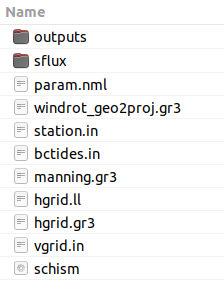
\includegraphics[width=0.3\textwidth]{figures/config.png}
    \caption{Example of directory for your run with mandatory and optional files for atmospheric forcing (sflux folder) and stations outputs}
    \label{fig:run}
\end{figure}
%%%%%%%%%%%%%%%%%%%%%%%%%%%%%%
\subsection{Mandatory file hgrid.gr3}
\noindent The horizontal grid can be created with different tools, a selection of which are listed in Table \ref{tab:grid gen}:
\begin{table}[htbp]
\centering
\caption{Grid generators}
\adjustbox{max width=\textwidth}{
\begin{tabular}{lccccc}
\hline
Name        & Node placement & Triangulation & Optimization & Boundaries & Availability \\ \hline
xmgredit    & Y              & Y             & Y            & Y          & Free         \\
SMS         & Y              & Y             & Y            & Y          & Commercial   \\
Gmsh        & Y              & Y             & Y            & Y          & Free         \\
OceanMesh2D & Y              & Y             & Y            & Y          & Free         \\
JIGSAW      & Y              & Y             & Y            & Y          & Free         \\
ADmesh      & Y              & Y             & Y            & Y          & Free         \\
BlueKenue   & Y              & Y             & Y            & N          & Free         \\
triangle    & Y              & Y             & N            & N          & Free         \\
nicegrid    & N              & N             & Y            & N          & Free        \\ \hline
\end{tabular}}
\label{tab:grid gen}
\end{table}\\
\noindent The specific aspect of gridgen using SMS is described in Chapter 5 of the manual, here we focus on BlueKenue. Interesting information for grid generation can also be found in Module T5 of the OPENCoast tutorials:\\
\url{http://opencoasts.lnec.pt/index_en.php#eventos}
%%%%%%%%%%%%%%%%%%%%%%%%%%%%%%%%%%%%%%%%%%%%%%%%%%%%%%%%%%
\subsubsection{Mesh creation with Blue Kenue}
\noindent First step is to download and install Qgis( Open source; Linux/Windows) and Blue Kenue (Open source; Windows-based application). For Blue Kenue:\\
\url{https://nrc.canada.ca/en/research-development/products-services/software-applications/blue-kenuetm-software-tool-hydraulic-modellers}\\
Then in Qgis you can import the shoreline for the area, adjust it to your domain and export it in a shapefile format. There are several sources to download shoreline in your areas of interest (Openstreetmap, NOAA with the Global Self-Consistent Hierarchical, High-resolution Geography Database, local navy charts etc...). Shapefile with coordinates in lon/lat can be saved in UTM using the option "save vector layer as CRS=..." (ex: 32755 for Tasmania).\\
In BlueKenue (BK), import the shapefile, create the domain with shoreline + additional lines, upload bathymetry (Digital Elevation Model) and generate your mesh following these tutorials (9 steps) on youtube:\\
\url{https://www.youtube.com/watch?v=hFUycwskJUo&t=2s}\\

Precision : once the coastline is appended in the domain, you may need to delete part of coastline to have only one line (no overlap between layers) at the same location (otherwise creation of error during the extraction).\\
Once your mesh is created you have to export it in SMS format(.2dm). Then you can convert it to .gr3 using the perl script "2dm2gr3\_m2m.pl" (link : $schism/src/Utility/SMS$) with the following commands:
\begin{lstlisting}[language=bash]
$ ./2dm2gr3_m2m.pl [version of SMS 0 1 2] [yourfile.2dm] [hgrid.gr3]
\end{lstlisting}
For the version of SMS from BK: 0 is working. For a quick check open the .gr3 file in  
xmgredit5 (you have to compile it before, see the file "install\_notes\_new" in $schism/src/Utility/ACE$), you will have an error if it's not correct. You can also check if there is the number of lines in the file corresponds to the number of elements directly by opening the file. \\
If your bathymetry is negative, transform it with xmgredit5:
\begin{lstlisting}[language=bash]
./xmgredit5 hgrid.gr3
\end{lstlisting}
Then: Edit/Edit over regions/Evaluate and then in the dialogue box type depth=depth*(-1).\\
Beware of CFL number condition, being an implicit model SCHISM require CFL$>$0.4 (see manual part 5.1.1 \& 5.1.2). The general rules are well explained in the section 5.1 of the manual.
%%%%%%%%%%%%%%%%%%%%%%%%
\subsubsection{Option optimization with nicegrid}
You can optimize your mesh with the tool nicegrid2 (\url{https://adcirc.org/home/related-software/adcirc-utility-programs/},download then compile), example is shown in Figure \ref{fig:nicegrid}.
\begin{figure}[htbp]
    \centering
    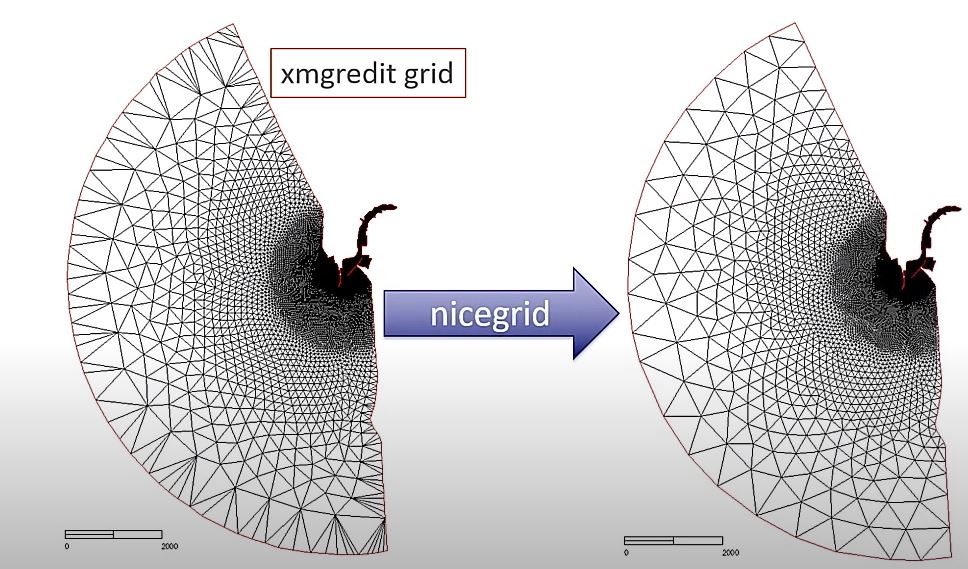
\includegraphics[width=0.9\textwidth]{figures/nicegrid2.JPG}
    \caption{Example of optimization of mesh with nicegrid (from Module T5 of OPENCoast Tutorials)}
    \label{fig:nicegrid}
\end{figure}
%%%%%%%%%%%%%%%%%
\subsubsection{Define boundaries}
\noindent Boundaries can be defined easily with xmgredit5. You have to define the boundaries (anti-clockwise) see this GIF for all the steps: \\
\url{http://ccrm.vims.edu/yinglong/feiye/Workshop_20190701/TEMP/Doc/hgrid.html}\\
Save file as bnb file. And check at the interface open bnd/land that the nodes are well defined.
%%%%%%%%%%%%%%
\subsubsection{Completion of hgrid.gr3, hgrid.ll as required for SCHISM}
\noindent You can create the lat/lon version of your grid from your UTM domain with another perl script "proj\_wrap.pl " ( Location: $schism/src/Utility/Pre-Processing$):
\begin{lstlisting}[language=bash]
$ ./proj_wrap.pl [epsg: "code zone of your area"]  [1: proj to ll; 2: ll to proj] 
[1: input format is .gr3; 2: input xyz] [file.gr3] [file.ll] 
[for xyz input, separator (1: space; 2: comma)] 
[for xyz input, line number (0: without; 1: with)]
#example:
$ ./proj_wrap.pl epsg:32755 1 1 hgrid.gr3 hgrid.ll 1 1 
\end{lstlisting}
The file hgrid.ll (coordinates in lat/lon) is mandatory for the creation of sflux files for atmospheric forcings.\\
Then merge hgrid.gr3 and hgrid.ll with the boundaries file created with xmgredit5:
\begin{lstlisting}[language=bash]
$ cat bnb >> hgrid.gr3
\end{lstlisting}
You're ready to check grid issues by running the pre-processor flag (ipre=1).
%%%%%%%%%%%%%%%%%%%
\subsection{Mandatory file vgrid.in}
\noindent The section 4.2.2 in the manual explained the different cases. Figure \ref{fig:vgrid} shows an example of a SZ model. For 2D barotropic model you can use the "pure S" model:
\begin{lstlisting}[language=bash]
2 !ivcor (SZ=2, LSC^2=1)
2 1 1.e6 ! Nz (# of Surface-levels), kz (# of Z-levels); h_s (transition depth between S and Z)
Z levels
1  -1.e6  ! coordinate of the last Z-level must match -h_s
S levels
40. 0. 1.e-4  ! constants used in S-transformation: h_c, theta_b, theta_f
   1    -1. !first S-level ( first sigma coordinate must be -1)
   2    0.  !last S-level ( last sigma coordinate must be 0)
\end{lstlisting}
\begin{figure}
    \centering
    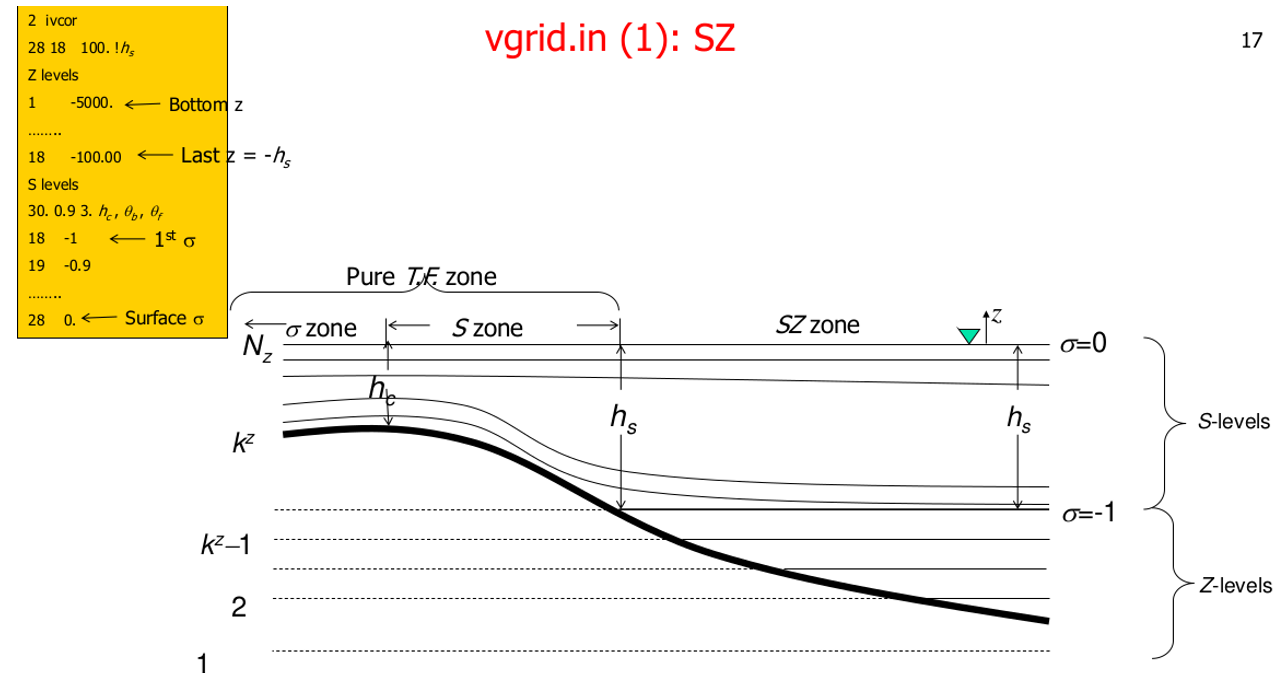
\includegraphics[width=0.9\textwidth]{figures/vgris_last.png}
    \caption{"vgrid.in" diagram}
    \label{fig:vgrid}
\end{figure}
%%%%%%%%%%%%%%%%%%%
\subsection{Mandatory file param.nml}
\noindent This file is well described in section 4.2.4 of the manual, and there are examples of this file in $schism/sample\_inputs$ and in the test suite "schism\_verification\_tests".
%%%%%%%%%%%%%%%%%%%
\subsection{Mandatory file bctides.in}
\noindent All the options supported by SCHISM are described in the section 4.2.3 of the manual. A good description of the file is available with this link:\\
\url{http://ccrm.vims.edu/yinglong/feiye/Workshop_20190701/TEMP/Doc/bc.html}
%%%%%%%%%%%%%%%%%%%%%%%%%%%
\subsubsection{Matlab}
\noindent You have a matlab code "one\_click\_bctides\_schism\_fes2014" in folder $schism/src/Utility/Tides$ to create bctides with FES2014 data. First you have to download the FES2014 data, e.g. from \url{https://www.aviso.altimetry.fr/en/data/products/auxiliary-products/global-tide-fes/}.
%%%%%%%%%%%%%%%%%%%%%%%%
\subsubsection{Python}
\noindent For TPXO there is the possibility to use pychsim developed by Jaime Cazalda:\\ \url{https://github.com/schism-dev/pyschism}\\
After installation, the cmd line to have information:
\begin{lstlisting}
$ pyschism  bctides -h
usage: pyschism bctides [-h] [--output-file OUTPUT_FILE] [--include-velocity]
 [--tidal-database {hamtide,tpxo}] [--Z0 Z0] [--hgrid-crs HGRID_CRS] 
 [--overwrite] [--log-level {critical,fatal,error,warn,warning,
   info,debug,notset,detail,partitioning}] hgrid start_date run_days

positional arguments:
  hgrid
  start_date
  run_days

optional arguments:
  -h, --help            show this help message and exit
  --output-file OUTPUT_FILE
  --include-velocity
  --tidal-database {hamtide,tpxo}, --tidal-db {hamtide,tpxo}
  --Z0 Z0
  --hgrid-crs HGRID_CRS
  --overwrite           Allow overwrite of output file.
  --log-level {critical,fatal,error,warn,warning,info,debug,notset,
  detail,partitioning}
  \end{lstlisting}
After downloading the data from TPXO (i.e. from \url{https://www.tpxo.net/}: h\_tpxo9.v1.nc and u\_tpxo9.v1.nc), copy the netcdf TPXO files to \$Home/.local/tpxo/*.nc and then you can create the "bctides.in" file:
\begin{lstlisting}
$ pyschism bctides [your file hgrid.ll] YYYY-MM-DDT00:00:00 
[number of days for simulation] --tidal-database=[your source] 
--include-velocity --output-file=bctides.in\\
Example:
$ pyschism bctides hgrid.ll 2018-03-01T00:00:00 7 
--tidal-database=tpxo --include-velocity --output-file=bctides.in
\end{lstlisting}
This will put into "bctides.in" for each constituent requested:
\begin{itemize}
    \item angular frequency and tidal species (not varying with time and space)
    \item nodal factor and earth equilibrium argument (varying with time)
    \item amplitude and phases of constituents at the boundaries (varying with space)
\end{itemize}
%%%%%%%%%%%%%%%%%%%%%%%
\subsection{Mandatory file "bed roughness".gr3}
\noindent Information at:\\
\url{http://ccrm.vims.edu/yinglong/feiye/Workshop_20190701/TEMP/Doc/other_gr3.html}
\url{http://ccrm.vims.edu/yinglong/feiye/Workshop_20190701/TEMP/Doc/rough.html}
\subsubsection{Manning.gr3}
\noindent For a constant value of the Manning number([n]=$s/m^{1/3}$) follow these steps (Figure \ref{fig:hgridman}):
\begin{itemize}
    \item open hgrid in xmgredit5
    \item Edit grid/region
    \item Evaluate
    \item depth={value of Manning's number $n$}
    \item save as manning.gr3
\end{itemize}
\begin{figure}
    \centering
    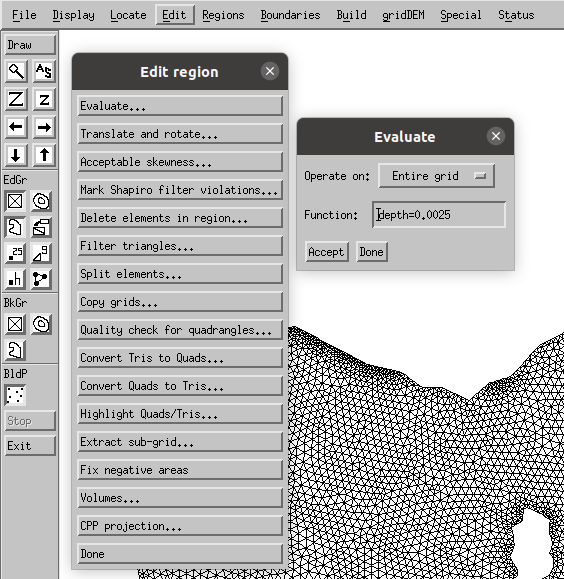
\includegraphics[width=0.9\textwidth]{figures/manning.png}
    \caption{Steps for the creation of manning.gr3}
    \label{fig:hgridman}
\end{figure}
You can also use BlueKenue to create a spatially varying Manning.gr3 (Credit to Huy Quang Tran). See the steps in the pdf under /src/Utility/Pre-Processing/step\_by\_step\_bottom\_friction\_BK.pdf.
\subsubsection{Rough.gr3}
Bottom roughness in meters are read from rough.gr3. [\textcolor{green}{from Joseph}: we've removed negative roughnes in newer versions like v5.9] In this case, negative or 0 depths in rough.gr3 indicate time-independent $C_D$, not roughness. With this option, two additional parameters are needed in param.nml: $dzb_{min}$ in meters and $dzb_{decay}$ nondimensional. Information can be found in the section 4.2.4.2 of the manual and in param.nml for the calculation of $C_D$ for rough.gr3:
\begin{lstlisting}
Cd is calculated using :
the log law, when dzb>=dzb_min; 
when dzb<dzb_min, Cd=Cdmax*exp[dzb_decay*(1-dzb/dzb_min)],
where Cdmax=Cd(dzb=dzb_min),
and dzb_decay (<=0) is a decay const specified below.
We recommend dzb_decay=0.
\end{lstlisting}
%%%%%%%%%%%%%%%%%%%%%%%%%%
\subsection{Optional files sflux.nc for atmospheric forcing}
\noindent The section 4.3.8 of the manual described how to generate your own sflux files with matlab, and gave the conventions for the nc files. \\
Others useful links: \\
\url{http://ccrm.vims.edu/w/index.php/Atmospheric_forcing}\\
\url{http://ccrm.vims.edu/yinglong/feiye/Workshop_20190701/TEMP/Doc/sflux.html}\\

\noindent Here is underlined the method to create sflux\_air only with python from GFS data.\\
%Get the files for hindcast:
%\urlstyle{https://www.ncei.noaa.gov/thredds/model/gfs.html}
%Analysis historical:
%\urlstyle{https://www.ncei.noaa.gov/thredds/catalog/model-gfs-g4-anl-files-old/catalog.html}
GFS data for SCHISM is available at \url{https://rda.ucar.edu/datasets/ds084.1/} (need to register for access), you need to have the start of your downloaded data file = start\_time of your simulation.\\
Grab the following fields:
\begin{itemize}
    \item wind speed (u,v) (10m above MSL)
    \item air pressure (MSL)
    \item surface air T (2m above MSL)
    \item specific humidity (2m above MSL)
\end{itemize}
Merge by time each variables with the command cdo (download from https://sourceforge.net/projects/cdo/):
\begin{lstlisting}
cdo mergetime gfs.0p25.*.f000.grib2.yourname.nc output.nc
\end{lstlisting}
Then merge all variables: 
\begin{lstlisting}
cdo merge [].nc [].nc [].nc sflux.nc
\end{lstlisting}
Then change the time units to "days since start\_date" with cdo  (before it was hours since 1880):
\begin{lstlisting}[language=bash]
cdo -setreftime,'2018-03-16','00:00:00' sflux.nc sflux_new.nc 
cdo -settunits,day sflux_new.nc sflux_air.nc 
OR in one command
cdo -setreftime,'2018-03-16','00:00:00',day sflux.nc sflux_air.nc 
\end{lstlisting}
Now you need to put all these variables in a new NetCDF compatible for SCHISM (sflux\_air\_1.0001.nc), using the script in Appendix A.1.
Put the file created in a folder "sflux" with a file "sflux\_inputs.txt" (In this file advanced users can specify parameters like renaming variable names, resetting max time window etc. Most users won't bother about these), and this folder in the folder of your run (Figure \ref{fig:sflux}).\begin{figure}[hbtp]
    \centering
    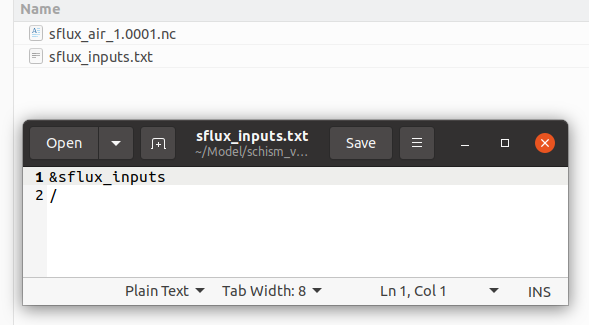
\includegraphics[width=0.6\textwidth]{figures/sflux.png}
    \caption{Example of contents for sflux folder, also showing the contents the file sflux\_inputs.txt}
    \label{fig:sflux}
\end{figure} \newline
Then create the file windrot\_geo2proj.gr3 : it's hgrid.gr3 with rotation value instead of depth . It rotates the wind in case they do not align with coordinates axes. If no rotation is needed put 0: you can use xmgredit5 for that by changing all values of 'depth' to 0 and saving it as windrotgeoproj.gr3.\\
If you use this option don't forget to put nws=2 in param.nml.

%%%%%%%%%%%%%%%%%%%%%%%%%%%%%%%%%%%%%%%%%%%%%%%%%%%%%
\subsection{Optional files elevation non tidal (2D): elev.th.nc}
\noindent Here is described the way to deal with global ocean (Mercator) data. First download the data, available through CMEMS Data Access Portal (\url{https://marine.copernicus.eu/}, need to register first):
\begin{itemize}
  %  \item 'thetao' (sea water potential temperature)
  %  \item 'so' (sea water salinity)
  %  \item 'uo' (eastward sea water velocity)
   % \item 'vo' (northward sea water velocity)
    \item 'zos' (sea surface height above geoid)
\end{itemize}
%(script "download-phys.py", just need to update the dates.)\\
Then change the reftime  to start\_time and units to seconds.
\begin{lstlisting}
cdo -setreftime,'YYYY-MM-DD','HH:MM:SS',second yourfile.nc elev.nc\
\end{lstlisting}
Run the python script "ElevUV\_bnb.py" (see Appendix A.2) to produce the "elev.th.nc" file for elevation. Then in bctides.in change the options for elevation: here 5 instead of 3, so the last line of Figure \ref{fig:caseBC} will become 748 5 3 0 0. Reminder all options for bctides are explained in table 4.1 of the manual.\\
\begin{figure}[htbp]
    \centering
    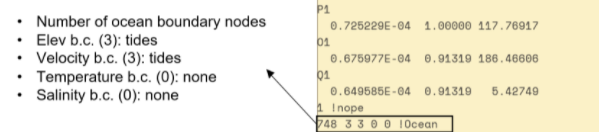
\includegraphics[width=0.8\textwidth]{figures/elevbc.png}
    \caption{Part of bctides.in to modify (from \url{http://ccrm.vims.edu/yinglong/feiye/Workshop_20190701/TEMP/Doc/bc.html})}
    \label{fig:caseBC}
\end{figure}
It's also possible to include non-tidal velocities by downloading eastward and northward velocities and creating "uv3D.th.nc". (Script in progress).

%%%%%%%%%%%%%%%%%%%%%%%%%%%%%%%%%%%%%%%%%%%%%%%%%%%%%
\subsection{Optional file stations.in}
This file is to  extract data (elev, air, pressure, windx, windy, T,S, u,v,w) at specific stations (model locations). The description can be found in section 4.3.7.1 of the manual.\\
Example:
\begin{lstlisting}[language=bash]
1 1 1 1 1 1 1 1 1   !on (1)|off(0) !flags for elev, air pressure, 
windx, windy, T, S, u, v, w
4                   !# of stations
1 6.5833 54.0000 0 !Format: station #,x,y,z; 
if ics=2, x,y are degr in lon/lat. #ics is defined in param.nml
2 7.1583 55.195 0 
3 6.35  54.1667 0 
4 8.4514 54.7942 0
\end{lstlisting}

%%%%%%%%%%%%%%%%%%
\section{Coupling with WWM (Wave Wind Model)}
\noindent There are three mandatory files for the WWM: 
\begin{itemize}
    \item wwminput.nml (equivalent of param.nml)
    \item wwmbnd.gr3 (file containing the description of the boundary condition)
    \item hgrid\_wwm.gr3 (copy of hgrid.gr3)
\end{itemize}
%%%%%%%%%%%%%%%%%%%%%%%%%%%%%%%%%%%%%%%%%%%%%
\subsection{Mandatory file wwminput.nml}
\noindent Example can be found in $schism/sample\_inputs$ for wwminput.nml. You have to update this file to match param.nml (i.e.: dtstep, start time of simulation), define your parameters, your option for wave forcing at the boundaries (IBOUNDFORMAT) and the start date of your wave forcing files. The manual under github (\url{https://github.com/schism-dev/schism/tree/master/src/WWMIII/Manual}) is obsolete for some sections, especially for the forcing part at the boundary (IBOUNDFORMAT). Two options are described here:
\begin{itemize}
    \item IBOUNDFORMAT=3 is for bulk parameters, requires 5 nc files (hs, t02, dir, spr, fp) and a parametric spectra is imposed along the open boundary considering a  JONSWAP spectrum or other.
    \item IBOUNDFORMAT=6 is for wave spectra from WWIII or any equivalent model able to produce the variables requested. One netcdf file with the following variables: 
    \begin{itemize}
    \item efth (directional variance spectral density) 
    \item dpt (depth)
    \item wnd (wind speed)
     \item wndir (wind direction)
     \item cur (current speed)
     \item curdir (current direction)
     \item frequency 1 (lower frequency)
     \item frequency 2 (higher frequency)
     \end{itemize}
\end{itemize}
%%%%%%%%%%%%%%%%%%%%%%%%
\subsubsection{Bulk parameters}
\noindent For IBOUNDFORMAT=3: write the name of the 5 nc files in a file called 'bndfiles.dat', \hl{the order is very important, to confirm someone? I have not yet managed to get this option to work in v5.8.}: \begin{enumerate}
    \item dir
    \item fp
    \item hs
    \item spr
    \item t02
\end{enumerate}
Copy these files in your folder for the run. Create wwwbnd.gr3 with python script (see Appendix A.3), and update param.nml to add the WWM global outputs: example in folder Test\_WWM\_Analytical (test suite : schism\_verification\_tests) and to ensure msc2 and mdc2 are equal to values in wwminput.nml.\\
Important items to check:
\begin{itemize}
    \item INITSTYLE= 1 (parametric Jonswap)
    \item LBCWA=T (Parametric Wave Spectra, T/F=TRUE/FALSE)
    \item LBCSP=F (Specify (non-parametric) wave spectra, specified in 'FILEWAVE' below),  T/F=TRUE/FALSE
\end{itemize}
%%%%%%%%%%%%%%%%%%%%%%%%
\subsubsection{Wave spectra}
\noindent With IBOUNDFORMAT=6, you have to specify for the item FILEWAVE the name of the netcdf with all the spectral data.\\
Important items to check:
\begin{itemize}
   \item INITSTYLE= 2 (read from global nc file you define in FILEWAVE)
    \item LBCWA= F (Parametric Wave Spectra)
    \item LBCSP= T (Specify (non-parametric) wave spectra, specified in 'FILEWAVE' below)
\end{itemize}

%%%%%%%%%%%%%%%%%%%%%
\subsection{Mandatory file wwmbnd.gr3}
\noindent For wwmbnd.gr3, it's a .gr3 style, you have to change the depth variable as follows:
\begin{enumerate}
    \item put 0 for every grid point (easily done with xmgredit5)
    \item put 1 for land boundary
    \item put -1 for island boundary
    \item put 2 for open boundary with Dirichlet conditions
    \item put 3 for open boundary with Neumann conditions (i.e. zero gradient)
\end{enumerate}
To create this file you can find a fortran script under github, a matlab script in the archives of schism\_users lists, and a python script in Appendix A.3.
There may be some duplicated nodes that are between land and open boundaries, you can manually work out to remove and keep the correct one.\\
%%%%%%%%%%%%%%%%%%%%%%%%%%%%%%%%%%%%%%%%%%
\subsection{Data for bulk parameters}
\subsubsection{Ifremer data}
%%%%%%%%%%%%%%%%%%%%%%%%%%%%%%%%%%%%
\noindent Ftp links must be open in a dedicated software (like filezilla for linux).\\ \url{ftp://ftp.ifremer.fr/}\\
Alternatively, an option is to download data (hs, fp , spr, t02, dir) with a bash script "get\_WW3.sh" (Credit to Ivica Janekovic):
\begin{lstlisting}
 # input argument is yyyy mm                                                    
 YEAR=$1
 MNTH=$2
 vars=( "fp" "dir" "hs" "t02" "spr" )
 for i in "${vars[@]}"
 do
 echo "getting $i for ${YEAR} ${MNTH}"
 wget -q --progress=dot "ftp://ftp.ifremer.fr/ifremer/ww3/HINDCAST/GLOBAL/${YEA\
R}_ECMWF/$i/WW3-GLOB-30M_${YEAR}${MNTH}_$i.nc" .
 echo "------------------------------------------------------------------------\
---------------------------------"
 done
\end{lstlisting}
cmd line:
\begin{lstlisting}
./get_WW3.sh 2018 03
\end{lstlisting}
(may need to do chmod +x get\_WW3.sh)\\
\noindent Then subset to your domain with:\\
ncks -dlatitude, min, max, stride -dlongitude, min, max, stride in.nc out.nc \\
Do this for each single variable nc file containing the entire period (not necessary to have the same start date as in param.nml).\\
In this example all variables are by month,  we have 2 files for Hs ( March and April)
\begin{lstlisting}
cdo mergetime inputs.nc output.nc
Ex: cdo mergetime hs_march.nc hs_april.nc hs_0304.nc
\end{lstlisting}
You have to do this for each variable and you will obtain 5 nc files which you have to put in the directory of your run (Figure \ref{fig:wavefolder}).
\begin{figure}[b!]
    \centering
    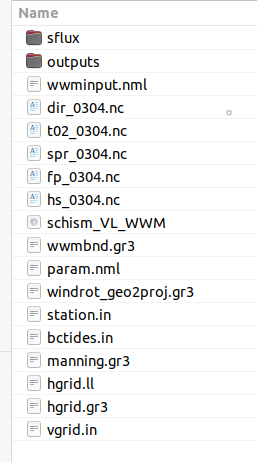
\includegraphics[width=0.4\textwidth]{figures/wavefolder.png}
    \caption{Configuration of SCHISM for coupling with waves and with atmospheric forcings}
    \label{fig:wavefolder}
\end{figure}

%%%%%%%%%%%%%%%%%%%%%%%%%%%%%%%%%%%%
\subsubsection{CAWCR data}
\noindent The Centre for Australian Weather and Climate Research (CAWCR) is a partnership between the Bureau of Meteorology and CSIRO. These wave fields are generated using the WWIII  model and the CFSR surface winds. \\
Link : \url{http://data-cbr.csiro.au/thredds/catalog/catch_all/CMAR_CAWCR-Wave_archive/CAWCR_Wave_Hindcast_aggregate/gridded/catalog.html}.\\
Input data: NCEP CFSR surface winds and sea ice, \url{http://cfs.ncep.noaa.gov/cfsr/}.\\
Wave model used: WaveWatch III, \url{http://polar.ncep.noaa.gov/waves/wavewatch/wavewatch.shtml}.\\

\noindent With Netcdfsubset you can subset to your domain and download nc files per month, for example "ww3.aus\_4m.YEARMONTH.nc"\\
You can download variables by variables or all variables in one file. If you download all variables together, to have each variable in a separate file (e.g. 1 file for hs, 1 file for dir etc.) you need to use the following commands:
\begin{lstlisting}
$ ncks -O -v hs gridded_ww3.aus_4m.201803.nc hs_03.nc #save only hs in new file
$ ncrcat hs_03.nc hs_04.nc hs_0304.nc #merge months
\end{lstlisting}

%%%%%%%%%%%%%%%%%%%%%%%
\subsection{Data for wave spectra}
The variables to download are:
\begin{itemize}
    \item efth (directional variance spectral density) 
    \item dpt (depth)
    \item wnd (wind speed)
     \item wndir (wind direction)
     \item cur (current speed)
     \item curdir (current direction)
     \item frequency 1 (lower frequency)
     \item frequency 2 (higher frequency)
\end{itemize}
\subsubsection{Ifremer data}
%%%%%%%%%%%%%%%%%%%%%%%%%%%%%%%%%%%%
\noindent Ftp links (\url{ftp.ifremer.fr}) must be open in a dedicated software (like filezilla for linux) or you can use the python script "ncget.py" in Appendix A.4.\\
Example of path: \\
$/ifremer/ww3/HINDCAST/GLOBMULTI\_ECMWF\_02/GLOB-30M/2018/SPEC\_SE$\\
Time period for:
\begin{itemize}
      \item ERA5: 1993-2020
    \item ECMWF: 2018-2019
\end{itemize}

%%%%%%%%%%%%%%%%%%%%%%%%%%%%%
\subsubsection{CAWCR data}
\noindent Spectra data can be found at :\\ \url{http://data-cbr.csiro.au/thredds/catalog/catch_all/CMAR_CAWCR-Wave_archive/CAWCR_Wave_Hindcast_aggregate/spec/catalog.html}\\
Time period: 1979-Jan to now

%%%%%%%%%%%%%%%%%%%%%%%%%%%%%%%%%%%%%%%%%%%%%%%%%%%%%%%%%%%%%%%%%%%%%%%%
\section{Post-processing}
\noindent The easiest way to visualize SCHISM nc4 outputs is decribed in section 5.3 of the manual: VisIT (you have to install it separately). Useful post-processing tools can be found in the $src/Utility$ directory and are described in the section 5.4 of the manual. Here some commands are detailed for the combination of nc4.
\begin{enumerate}
  \item to work with VisIT tool\\
Use the combine\_ouptut11.f90 (need to compile it first, follow instruction in the header of the file). Then in the outputs directory of your run:
\begin{lstlisting}[language=bash]
outputs$ ./combine_output11 -b [start number of output file] 
-e [end number of output file] 
outputs$ ./combine_output11 -b 1 -e 5 #example
\end{lstlisting}
This means that files schout\_0000\_1.nc, schout\_0000\_2.nc etc will become schout\_1.nc etc see Figure \ref{fig:visit}. For more information on partitioning (4-digit zeros) see the manual section 4.4.2. Then you can launch VisIT to visualize the results (Figure \ref{fig:visit} ):
\begin{lstlisting}[language=bash]
.../visit/bin$ ./visit
\end{lstlisting}
    \item to work with python, you can use the following command to deal with one file
\begin{lstlisting}[language=bash] 
outputs$ ncrcat schout_0000_[123456789].nc schout_combine.nc
\end{lstlisting}
\end{enumerate}
\begin{figure}[htbp]
    \centering
    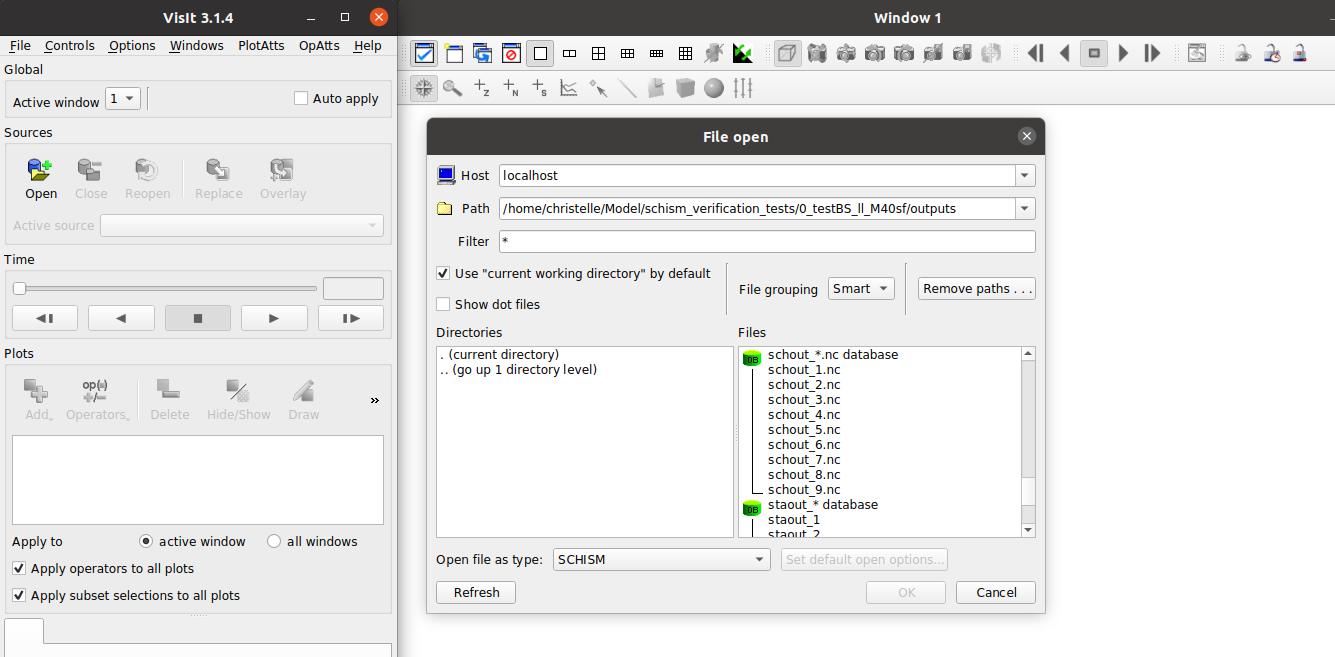
\includegraphics[width=0.9\textwidth]{figures/visitgood.png}
    \caption{Screenshot for opening a file in VisIT}
    \label{fig:visit}
\end{figure}
%%%%%%%%%%%%%%%%%%%%%%%%%%%%%%%%%%%%%%%%%%%%%%%%%%%%%%%%%%%%%%%%%%%%%%%%
\section{Full example for 2D model barotropic with tide forcing}
\noindent -Install and compile SCHISM to get schism.exe\\
-Install tools for pre-processing : xmgredit5, Qgis, Blue Kenue\\
-Create your mesh in Blue Kenue, export it in SMS format, convert it to .gr3 with perl script (Figure \ref{fig:hgrid})\\
-Create your vertical grid vgrid.in with example given in the manual\\
-Create bctides.in with pyschism (Figure \ref{fig:bct})\\
-Create your bottom drag file : manning.gr3\\
-Create your file station.in if needed\\
-Create your param.nml from template \\
-Put all of these files in a directory for your run\\
-Create a folder inside called outputs (see Figure \ref{fig:configS})\\
-You're ready to test your mesh with ipre=1 in param.nml (you can do this step as soon as you have your mesh ready)\\
-It's successful? So you can now run your simulation with ipre=0
-And you can see the files in outputs following a successful run in Figure \ref{fig:outputs}. 
Here the full example for 2D model barotropic with tide forcing was created to develop a tidal model for Banks Strait in Bass Strait, Tasmania. And we aimed to obtain elevation and depth-averaged velocities in all domain and at specific stations (= location of ADCP data).\\
Global output is done every "nspool" steps, and a new output stack is opened every "ihfskip" steps (these parameters are defined in param.nml), you obtained schout\_0000\_1.nc etc. The files staout\_1 etc are the outputs for the stations you defined in stations.in. Mirror.out, fatal.error, nonfatal\_0000 are main diagnostic output files.\\

\begin{figure}
    \centering
    \begin{minipage}[b]{0.45\textwidth}
        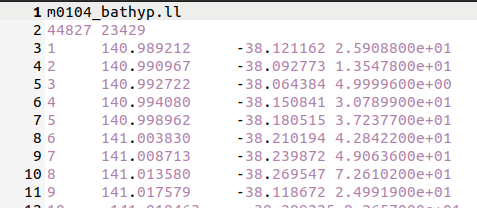
\includegraphics[width=\textwidth]{figures/hgrid.png}
    \caption{Start of hgrid.gr3 file}
    \label{fig:hgrid}
    \end{minipage}
\hfill
    \begin{minipage}[b]{0.45\textwidth}
    \centering
    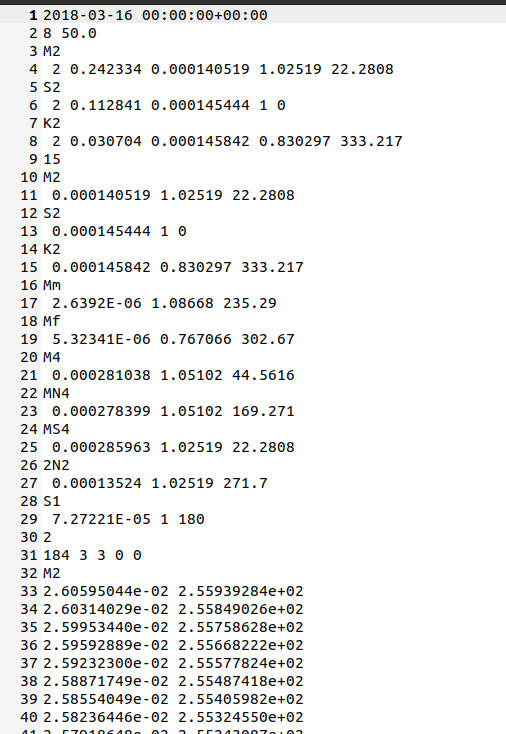
\includegraphics[width=\textwidth]{figures/bctide.png}
    \caption{Start of bctides.in file}
    \label{fig:bct}
    \end{minipage}
\end{figure}
\begin{figure}
    \centering
    \begin{minipage}[b]{0.45\textwidth}
        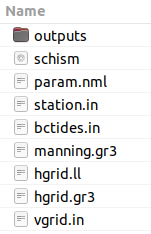
\includegraphics[width=0.7\textwidth]{figures/configsimple.png}
    \caption{Configuration for 2D barotropic with only tidal forcing}
    \label{fig:configS}
    \end{minipage}
\hfill
    \begin{minipage}[b]{0.45\textwidth}
    \centering
    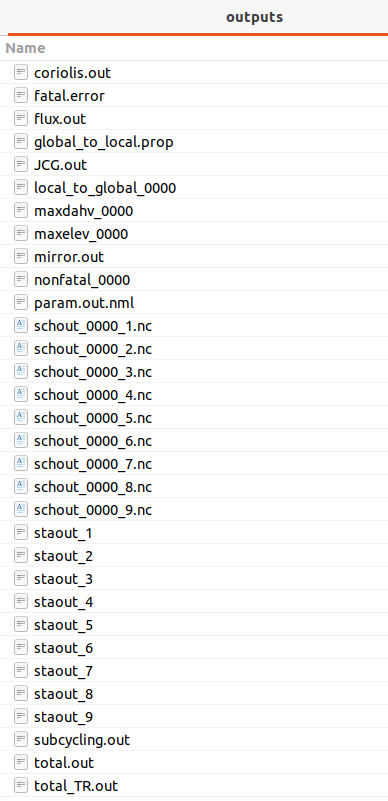
\includegraphics[width=\textwidth]{figures/outputs.png}
     \caption{Contents of outputs folder for 2D barotropic run with only tidal forcing}
     \label{fig:outputs}
    \end{minipage}
\end{figure}

%%%%%%%%%%%%%%%%%%%%%%%%%%%%%%%%%%%%%%%%%%%%%%%%%%%
\section{Error messages when running simulations}
\subsection{sflux files}
\begin{lstlisting}
0: ABORT:  Could not find suitable element in input grid for output node 
# 1 x_out, y_out =    2.6708680168154237
-0.47438771635516203      
in_elem_for_out_node, ae_min =            0   1.0000000000000001E+025  
\end{lstlisting}
This imply x1,x2,x3 are opposite, i.e. clockwise instead of anticlockwise in your input grid sflux.\\
\newline
\clearpage
%%%%%%%%%%%%%%%%%%%%%%%%%%%%%%%%%%%%%%%%%%
\acknowledgments{Thanks to Xavier Bertin, Joseph Zhang, Vanessa Hernaman, Jerome Lefevre, Ivica Janekovic, Jaime Calzada, Huy Quang Tran and Roger Proctor. }


%%%%%%%%%%%%%%%%%%%%%%%%%%%%%%%%%%%%%%%%%%
%% optional
\appendixtitles{no} %Leave argument "no" if all appendix headings stay EMPTY (then no dot is printed after "Appendix A"). If the appendix sections contain a heading then change the argument to "yes".
\appendix
\section{}
These scripts are in Github: \url{https://github.com/Krys1202/Guide_SCHISM/tree/main/Python_scripts}
\unskip
\subsection{Python script to create sflux air 1.0001.nc}
\begin{minted}{python}
#!/usr/bin/env python3
# -*- coding: utf-8 -*-
"""
Created on Wed Apr 21 14:41:09 2021
@author: Christelle Auguste inspired by "gfs.py" from pyschism and matlab scripts in src/Utility
"""
from netCDF4 import Dataset,num2date
from datetime import datetime
import numpy as np

#define your domain
lon_points = np.arange(lon value,lon value,0.25)
lat_points = np.arange(lat value,lat value,0.25)
lon , lat = np.meshgrid(lon_points, lat_points)

##create new netcdf
filename = 'sflux_air_1.0001.nc'
#nc = Dataset(filename, 'w', format='NETCDF4')
nc = Dataset(filename, 'w', format='NETCDF3_CLASSIC')
nc.setncatts({"Conventions": "CF-1.0"})
nc.createDimension('time', None)
nc.createDimension('ny_grid', len(lat_points)) 
nc.createDimension('nx_grid', len(lon_points)) 

lon_var = nc.createVariable('lon', np.float32, dimensions=('ny_grid','nx_grid'),)
lon_var[:]= lon
lon_var.units = 'degrees_east'
#lon_var.axis = 'X' # Optional
lon_var.standard_name = 'longitude'
lon_var.long_name = 'Longitude'

lat_var = nc.createVariable('lat', np.float32, ('ny_grid','nx_grid'),)
lat_var[:] = lat
lat_var.units = 'degrees_north'
#at_var.axis = 'Y' # Optional
lat_var.standard_name = 'latitude'
lat_var.long_name = 'Latitude'


time_units='days since 20XX-XX-XX'
time_var = nc.createVariable('time', np.float32, ('time',))
time_var.units = time_units
#time_var.axis = 'T'  # Optional
time_var.standard_name = 'time' 
time_var.long_name = 'Time'
time_var.base_date=(20XX, XX, XX, 0)

prmsl_var = nc.createVariable('prmsl', datatype=np.float32,
                              dimensions=('time', 'ny_grid', 'nx_grid'),
                              zlib=True)
prmsl_var.units = 'Pa'
prmsl_var.standard_name = 'Pressure reduced to MSL'
prmsl_var.long_name = 'air_pressure_at_sea_level'
prmsl_var.missing_value = -9999

uwind_var = nc.createVariable('uwind', datatype=np.float32,
                              dimensions=('time', 'ny_grid', 'nx_grid'),
                              zlib=True)
uwind_var.units = 'm/s'
uwind_var.standard_name = 'eastward_wind'
uwind_var.long_name = 'Surface Eastward Air Velocity (10m AGL)'

vwind_var = nc.createVariable('vwind', datatype=np.float32,
                              dimensions=('time', 'ny_grid', 'nx_grid'),
                              zlib=True)
vwind_var.units = 'm/s'
vwind_var.standard_name = 'northward_wind'
vwind_var.long_name = 'Surface Northward Air Velocity (10m AGL)'

stmp_var = nc.createVariable('stmp', datatype=np.float32,
                              dimensions=('time', 'ny_grid', 'nx_grid'),
                              zlib=True)
stmp_var.units = 'K'
stmp_var.standard_name = 'air_temperature'
stmp_var.long_name = 'Surface Air Temperature (2m AGL)'

spfh_var = nc.createVariable('spfh', datatype=np.float32,
                              dimensions=('time', 'ny_grid', 'nx_grid'),
                              zlib=True)
spfh_var.units = '1'
spfh_var.standard_name = 'specific_humidity'
spfh_var.long_name = 'Surface Specific Humidity (2m AGL)'
    
#Fill the new nc file with GFS 0.25deg data (combined in one nc file)
d  = Dataset('sflux_air.nc')    
tvar = 'initial_time0_hours'
t = d[tvar][:]
t_unit = d.variables[tvar].units
print(t_unit)
tvals = num2date(t,units = t_unit)

str_t = [i.strftime('%Y%m%d %H%M') for i in tvals] 
#to display dates as string
datetime_t = [datetime.strptime(i,"%Y%m%d %H%M") for i in str_t]
# print(str_t)
# print(datetime_t)
time_var[:]= t

pvar = 'PRMSL_P0_L101_GLL0'
prmsl=d[pvar][:][:][:]
print(prmsl.shape)
prmsl_var[:,:,:] = prmsl 

uvar = 'UGRD_P0_L103_GLL0'
uwind = d[uvar][:][:][:]
print(uwind.shape)
uwind_var[:,:,:] = uwind 

vvar = 'VGRD_P0_L103_GLL0'
vwind = d[vvar][:][:][:]
print(vwind.shape)
vwind_var[:,:,:] = vwind 

sphvar = 'SPFH_P0_L103_GLL0'
sph = d[sphvar][:][:][:]
print(sph.shape)
spfh_var[:,:,:] = sph

stmpvar = 'TMP_P0_L103_GLL0'
stmp = d[stmpvar][:][:][:]
print(stmp.shape)
stmp_var[:,:,:] = stmp 
d.close()
nc.close()
\end{minted}
\clearpage
%%%%%%%%%%%%%
\subsection{Python script to create elev2D.th.nc}
\begin{minted}{python}

#!/usr/bin/env python3
# -*- coding: utf-8 -*-
"""
Created on Tue May  4 11:42:35 2021

@author: christelle
"""
from netCDF4 import Dataset,num2date
from datetime import datetime
import numpy as np
import xarray as xr
#import pandas as pd

# get lon/lat of open boundaries nodes from hgrid.ll
f=open('hgrid_principal.ll','r')
data=f.readlines()

num_nodes_and_elements = data[1]
num_nodes = num_nodes_and_elements.split(" ")[1]
num_elements= num_nodes_and_elements.split(" ")[0]

nodes_start = 2
node_lines = data[nodes_start:nodes_start+int(num_nodes)]

elements_start = nodes_start + int(num_nodes) 
element_lines = data[elements_start:elements_start + int(num_elements)]

metadata1_start = elements_start + int(num_elements) 
metadata1_line = data[metadata1_start:metadata1_start + 3]
metadata_obnb=data[metadata1_start+1]
numnodes_obnb=metadata_obnb.split(" ")[0] #to have total number of nodes in open bnd
metadata_obnb1=data[metadata1_start+2]
numnodes_obnb1=metadata_obnb1.split(" ")[0] 

obnodes1_start =metadata1_start+ 3
obnnode1_lines=data[obnodes1_start:obnodes1_start+int(numnodes_obnb1)]

metadata2_start = obnodes1_start + int(numnodes_obnb1)
metadata_obnb2=data[metadata2_start]
numnodes_obnb2=metadata_obnb2.split(" ")[0]

#only one open bnd in this case
# obnodes2_start =metadata2_start+ 1
# obnnode2_lines=data[obnodes2_start:obnodes2_start+int(numnodes_obnb2)]


openbnd_lines=obnnode1_lines#+obnnode2_lines #all the lines for all nodes in open bnd

#get the coordinates corresponding to the open bnd nodes
bnd_coord=[]
nodeLon=[]
nodeLat=[]
nodeLont=[]
nodeLatt=[]
for i in range(len(openbnd_lines)):
        node_index = int(openbnd_lines[i])
        node= node_lines[node_index-1]
        #node_num=node[0:5]
        node_lont=node.split(" ")[5]
        node_latt=node.split(" ")[10]
        #append lon, lat
        nodeLont.append(node_lont)
        nodeLatt.append(node_latt)

bnd_coord= np.column_stack([nodeLont, nodeLatt])

nOpenBnbNodes=int(numnodes_obnb)

##create new netcdf elev2D.th.nc
filename = 'elev2D_RES.th.nc'
nc_elev = Dataset(filename, 'w', format='NETCDF4')
#nc_elev = Dataset(filename, 'w', format='NETCDF3_CLASSIC')
nc_elev.setncatts({"Conventions": "CF-1.0"})
nc_elev.createDimension('time', None)
nc_elev.createDimension('nComponents', 1) 
nc_elev.createDimension('nLevels', 1) 
nc_elev.createDimension('nOpenBndNodes', len(bnd_coord)) #nOpenBnbNodes
nc_elev.createDimension('one', 1) 

one=1

time_var = nc_elev.createVariable('time', np.double, ('time',))
time_var.units = 's'
time_var.long_name = 'simulation time in seconds'


timestep_var = nc_elev.createVariable('time_step', np.float32, 'one')
timestep_var.units = 's'
timestep_var.long_name = 'time step in seconds'
timestep_var[:]= 86400


elev_var = nc_elev.createVariable('time_series',np.float32,('time','nOpenBndNodes',
                              'nLevels', 'nComponents'),)
elev_var.long_name = 'elev_nontidal'
elev_var.units='m'



################Fill the new nc files with Mercator data ( ex 1month  01/07/2018)
d  = Dataset('merc-all-201012-1bis.nc') #modified from original version with 
#cdo to have time in seconds
tvar = 'time'
t = d[tvar][:]
t_unit = d.variables[tvar].units
#print(t_unit)
tvals = num2date(t,units = t_unit)
str_t = [i.strftime("%Y%m%d %H%M") for i in tvals] # to display dates as string
datetime_t = [datetime.strptime(i,"%Y%m%d %H%M") for i in str_t]
time_var[:]= t


######### need to find the values for lon/lat of openbnb =bnd_coord

nc=xr.open_dataset('merc-all-201012-1bis.nc') 
subset=nc.sel(longitude=bnd_coord[:,0], latitude=bnd_coord[:,1], method='nearest')
SSH=nc.zos
# #########elev2D
elev_test=subset.zos.values
elev_test2=np.zeros([len(t),len(bnd_coord)])

for j in range(len(t)):
    for i in range(len(bnd_coord)):
      elev_test2[j,i] = elev_test[j,i,i]

#put nan values=0
elev_nonan=np.nan_to_num(elev_test2)
SE_RES=np.mean(elev_nonan)
SSH=elev_nonan-SE_RES

elev_var[:,:,:,:] = SSH



d.close()
nc_elev.close()


\end{minted}
\clearpage
%%%%%%%%%%%%%%%%%%%%%%%%%%%%%%%%%%%%%%%%%%%%%%%%%%%%%%%%%%%%%%%%%%%%%%%%%%%%%%%%%
\subsection{Python script to create wwmbnd.gr3}
\begin{minted}{python}
#Create wwmbnd.gr3 based on SELFE open bnd segments
import csv
import numpy as nu

#     Inputs:         
#     hgrid.gr3, 
#     gen_wwmbnd.in (see sample below)

#     Output: wwmbnd.gr3

#     python create_wwmbnd_gr3.py
	
#     Sample gen_wwmbnd.in
#4 !ncond, i.e. number of conditions
#1 2 2 !cond1 #seg flag ob
#2 2 1 !cond2 #seg flag land
#3 22 -1 !cond3 #seg flag island
#4 99 0 !cond4 #dummy flag other nodes
	
#     Input files, info about flags for different boundaries
#     conditions ordered as they appear in hgrid.gr3
#     i.e. open, land, island
#     condition #, # boundaries, flag for open boundary nodes
#     condition #, # boundaries, flag for land boundary nodes
#     condition #, # boundaries, flag for island boundary nodes
#     condition #, # boundaries, flag for other nodes (set inside code as initial condition)

f = open('gen_wwmbnd.in')
bnd_in = f.readlines()
f.close()

ncond = int(bnd_in[0][0])
print('number of node condition flags is',ncond,' these are:')
for i in range(ncond):
    ii=i+1
    x = bnd_in[ii].split(' ')
    #print(x)
    print(f'condition {x[0]}, # boundaries {x[1]}, flag {x[2]}')

#read in details from hgrid
with open('hgrid.gr3') as f:
    fr = csv.reader(f,delimiter=' ')
    next(fr)
    nenp = next(fr)
    #initialise arrays (ne = number of elements; np = number of nodes)
    #xnd = lond, ynd = lat, ibnd = node number, nm = 3 nodes numbers per element 
    ne = int(nenp[0])
    np = int(nenp[1].strip())
    xnd =nu.zeros([np])
    ynd =nu.zeros([np])
    ibnd=nu.zeros([np], dtype='i')
    nm=nu.zeros([ne,3], dtype='i')

    print(ne,np,nm.shape)

    #read in xnd,ynd for each node
    for i in range(np):
        rec=next(fr)
        #print(rec)
        k=0
        for j in range(len(rec)):
            if rec[j] !='':
                if k == 1: xnd[i] = float(rec[j])
                if k == 2: ynd[i] = float(rec[j])
                k=k+1
    print(xnd[0],ynd[0])

    #read in node numbers for each element 
    for i in range(ne):
        rec = next(fr)
        if i==0: print(rec)
        for j in range(2,5):
            m = int(rec[j])
            nm[i,j-2] = m
            if i==0: print(rec,j,m,nm[i,j-2])

    print(nm[0,:],nm.dtype)


    rec = next(fr)
    nope = int(rec[0])
    print(nope)

    #check expected number of open boundaries
    x = bnd_in[1].split(' ')
    nope2 = int(x[1])
    if nope!=nope2: 
        print('nope/=nope2')
        exit()

    #ok, set up flag
    ifl_ob = int(x[2])

    neta = next(fr)

    for k in range(nope):
        rec=next(fr)
        nond = int(rec[0])
        print(nond)
        for i in range(nond):
            rec = next(fr)
            iond = int(rec[0])
            if i == 0: print(rec,iond)
            if iond>np or iond<=0:
                print('iond>np')
                exit()
            ibnd[iond-1]=ifl_ob

    #now land/island boundaries
    #total number of land/island boundaries
    rec = next(fr)
    nlandb = int(rec[0])
    #total number of land boundary nodes
    rec = next(fr)
    nlandn = int(rec[0])
    print('number of land/island boundaries',nlandb)
    print('number of land nodes',nlandn)

    #check expected number of land boundaries
    x2 = bnd_in[2].split(' ')
    x3 = bnd_in[3].split(' ')
    print(x2)
    print(x3)
    nlb = int(x2[1]) #number of land boundaries
    nib = int(x3[1]) #number of island boundaries
    nlib = nlb+nib
    if nlandb!=nlib: 
        print('nlandb/=nlb',nlandb,nlib)
        exit()

    ifl_l = int(x2[2])
    ifl_i = int(x3[2])
    print('flags for land and island',ifl_l,ifl_i)

    for k in range(nlandb):
        rec = next(fr)
        nond = int(rec[0])
        print(nond)
        for i in range(nond):
            rec = next(fr)
            iond = int(rec[0])
            if i == 0: print(rec,iond)
            if iond>np or iond<=0:
                print('iond>np')
                exit()
            #check if land or island boundary
            if k <= nlb-1:
                ibnd[iond-1]=ifl_l
            else:
                ibnd[iond-1]=ifl_i

#
#     Output
#
#     Output file
with open('wwmbnd.gr3','w') as w:
    ww = csv.writer(w,delimiter=' ')
    ww.writerow('')
    ww.writerow([ne,np])
    for i in range(np):
        ww.writerow([i+1,xnd[i],ynd[i],float(ibnd[i])])
    for i in range(ne):
        ww.writerow([i+1,3,nm[i,0],nm[i,1],nm[i,2]])

# check duplicated nodes, and check for the first node of open 
# bnd

\end{minted}
\clearpage
%%%%%%%%%%%%%%%%%%%%%%%%%%%%%%%%%%%%%%%%%%%%%%%%%%%%%%%%%%%%%%%%%%%%%%%%%%%%%%%%%%
\subsection{Python script to download Ifremer spectral data (ncftpget.py) }
\begin{minted}{python}
import subprocess
year = 2018
lats = [54.0]
lons = [2.5]
model = 'GLOB-30M'
fils = f'WW3-{model}-'
filf = '_spec.nc'

k=0
for lo in lons:
    lon = lo*10
    lon = str(int(lon)).zfill(4)
    print(lon)
    for la in lats:
        ifail=0
        lat = la*10
        lat = str(int(lat)).zfill(3)
        print(lat)
        fil = f'{fils}E{lon}S{lat}_{year}{filf}'
        print(fil)
        #ftp://ftp.ifremer.fr/ifremer/ww3/HINDCAST/GLOBMULTI_ECMWF_02/GLOB-30M/
        #2018/SPEC_SE/WW3-GLOB-30M-E0000S680_2018_spec.nc
        cmd =
        f'ncftpget ftp://ftp.ifremer.fr/ifremer/ww3/HINDCAST/GLOBMULTI_ECMWF_02/{model}/{year}/SPEC_SE/{fil}'
        print(cmd)
        ifail = subprocess.call(cmd,shell=True)
        if ifail != 0:
            print(f'{fil} not found')
        #if k==0:exit()

\end{minted}
%=====================================
% References, variant B: external bibliography
%=====================================
\externalbibliography{yes}
\bibliography{BibTeX_file}


%%%%%%%%%%%%%%%%%%%%%%%%%%%%%%%%%%%%%%%%%%
\end{document}

